% TODO: Ez elé még érdemes lenne összegyűjteni, hogy milyen hasonló játékok vannak. Melyek az azokból preferált elemek, illetve hangsúlyozni kellene, hogy milyen szempontból próbál egyedi lenni a játék. -

\Chapter{Koncepció}

A játék bizonyos játékokból már ismert elemeket tartalmaz, ilyen pédául a Pixel Dungeon és Darkest Dungeon-ből már ismert folyosó-szoba kapcsolat, ahol a dungeon több különböző szobából épül fel, amelyeket folyosók kötnek össze. A Darkest Dungeon-nel ellentétbnen, arra törekszünk, hogy a játékos ne legyen lekorlátozva az adott szobára 'combat' közben.
De milyen szempontokból is próbál egyedi lenne a játék? A hangsúly a környezetünk nagyobb bevonása a 'combat' fázisba és a 'combat' átdolgozása olyanannyira hogy elég komplex legyen az ideális lépések megtalálása.
A játékot röviden, nagyjából összefoglaló folyamatábra amelyben a közelharc szekvenciát részleteztük egy új folyamatábrában a láthatóság kedvéért. Combat folyamatábra (\ref{fig:combat}. ábra).

\begin{figure}[h!]
	\centering
	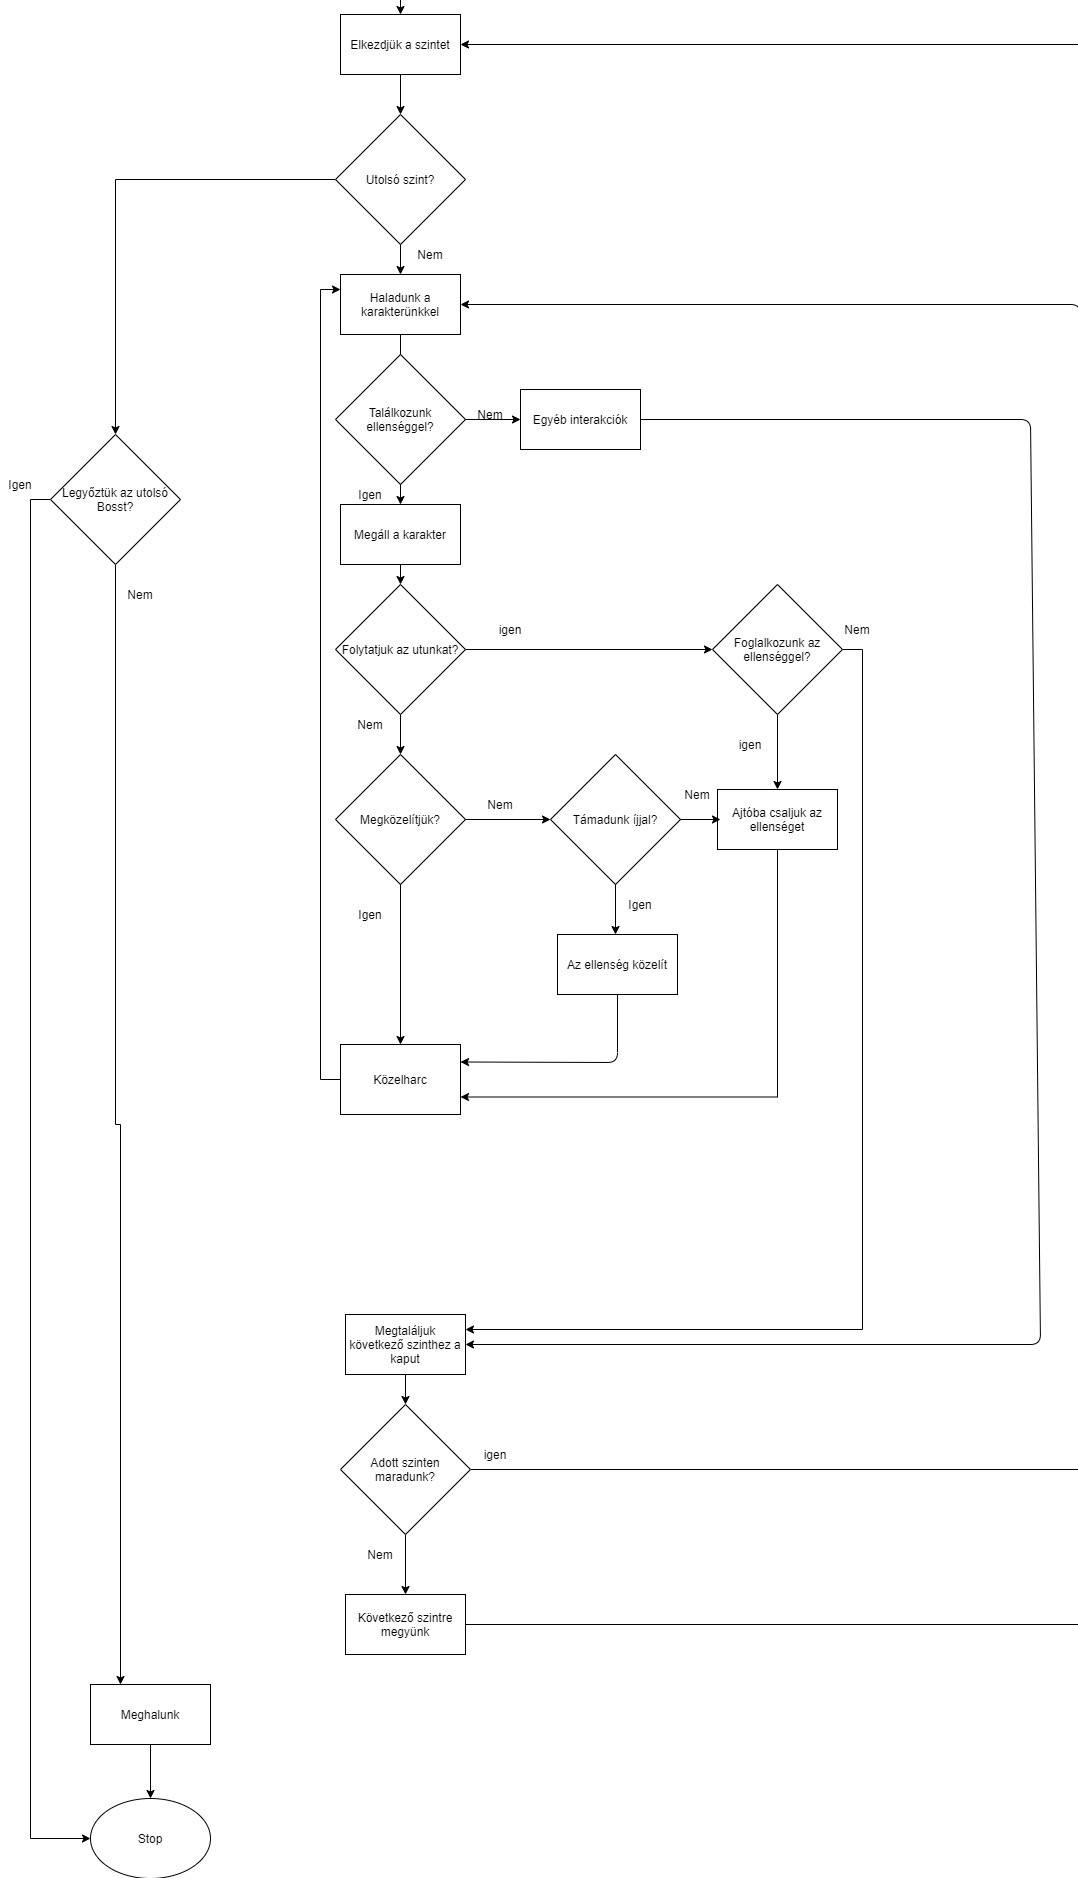
\includegraphics[width=\textwidth]{images/image1.png}
	\caption{Combat folyamatábra}
	\label{fig:combat}
\end{figure}

\Section{Menü}

A játék indításakor vagy megállításakor felugró ablak.
Start/Continue:
A játék indításakor a menüben a start-ot látjuk, ha a játékot állítjuk meg, akkor a menüben a continue-t látjuk.
Ezen menüpont kiválasztásával kezdhetjük a játékmenetünket vagy folytathatjuk azt.
Save:
Ez a menüpont nem jelenik meg a játék indításakor csak akkor, hogyha játékmenetet állítunk meg.
Ezen menüpont kiválasztásával menthetjük a jelenlegi játékmenetünket.
Load:
Ezen menüpont mindig jelen van a menüben, elérhető a játék indításakor és megállításakor is.
Ezen menüpont kiválasztásával tölthetjük be az általunk lementett mentéseket.
Options:
Ezen menüpont mindig jelen van a menüben, elérhető a játék indításakor és megállításakor is.
Ezen menüpont kiválasztásával egy új ablakra irányít át minket.
Itt lehetőségünk van hangbeállítások személyre szabására, mint például a zene és a játékbeli hangok. (Több csúszka segítségével)
Lehetőségünk van fényerő beállításokra is, mint például a Gamma állítására. (Egy csúszka segítségével)
Nyelvi beállítások a menüre vonatkozóan. (Legördülő fülből kiválasztva)
Vér ki/bekacsolása játék közben. (Egy ki/bepipálható rublika)
Végezetül egy visszagomb ami visszairányít minket a menübe.
Rankings(history):
A főmenüben található rákattintásakor felugrik egy ablak amiben összes régebbi karakterünk alapstatisztikáit kilistázza.
Badges(achievements):
Szintén a főmenüből elérhető, megnyitásakor a játékban szerzett cselekedeteink után kapunk jelvényeket.
Log out:
Kiléptet minket a jelenlegi fiókunkból, visszairányítva a bejelentkezési ablakhoz.
A log-out a menüben mindig szerepel.
Main menu:
Ez a gomb akkor szerepel a menüben hogyha egy játékmenet megállításával kerülünk a menübe.
Ez befejezi a jelenlegi játékmenetünket és visszaírányít minket a főmenübe.

\begin{figure}[h!]
	\centering
	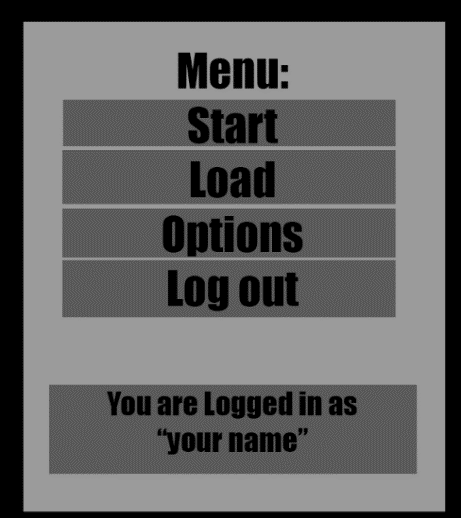
\includegraphics[scale=1]{images/image2.png}
	\caption{Főmenü}
	\label{fig:image2}
\end{figure}

\begin{figure}[h!]
	\centering
	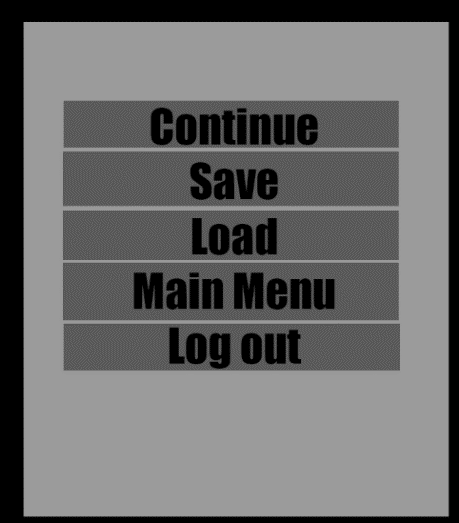
\includegraphics[scale=1]{images/image3.png}
	\caption{Játékbeli menü}
	\label{fig:image3}
\end{figure}

\begin{figure}[h!]
	\centering
	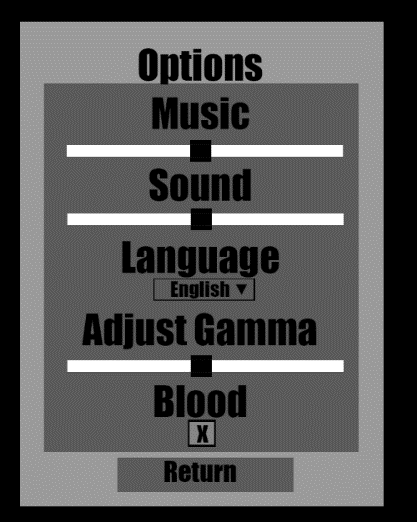
\includegraphics[scale=1]{images/image4.png}
	\caption{Options}
	\label{fig:image4}
\end{figure}

Ahol a Fekete háttér, az a megállított játék képe lenne elhomályosítva.
Ha még nem kezdtünk bele egy játékmenetbe, akkor pedig általunk megadott játékmenet képernyőmentése lenne a háttérben elhomályosítva.

\Section{Map}

% TODO: A map-ek szerkezetéről részletesebben írni kellene. Feltételezhetően egy mátrixról van szó, amelynek a celláit itt blokknak nevezzük. Le kellene írni konkrétan az egy-egy blokkhoz tartozó adatokat.

A map szobák és folyosók összesége, ahol a szobák alakjánál törekszünk a négyzet alakú szobák elkerülésére. A folyosók vagy 'I', 'Y' vagy 'L' ...stb alakot követik. A szobákban és a folyosókban bejárható terület egy mátrixhoz hasonló, ahol a celláit blokkoknak nevezzük.
Minden blokkhoz tartoznak adatok.
Ezek az adatok:
\begin{itemize}
    \item X koordináta (egészérték)
    \item Y koordináta (egészérték)
    \item Bejárhatóság (Boolean típusú érték, azt vizsgálja, hogy bejárható az adott blokk)
    \item Tárgy (intiger típúsú tömb, az adott blokkon lévő tárgyak ID-t tartalmazza)
    \item Effekt (intiger típúsú tömb, az adott blokkon lévő effektek ID-t tartalmazza)
    \item Entity (Boolean típusú érték, azt vizsgálja, hogy az adott blokkon van-e Entity)
\end{itemize}

% TODO: A map-ek közötti kapcsolódási pontokat jobban részletezni kellene, és úgy általában a map-en való mozgást.

A játékmenet egy szobában kezdődik. Amelyeken ajtók vannak. Minden szobából az ajtók egy folyosóra nyílnak. Szobák közötti mozgást a folyósókon való mozgással tehetjük meg.

% TODO: Hogy ha az egymás melleti blokkokra vonatkozóan meg lehet adni valamilyen előírásokat, akkor azt is érdemes részletezni.

Fontosabb kizáró feltételek:
\begin{itemize}
    \item Ajtók egymás mellett közvetlenül.
    \item Folyosóból ne nyíljon ajtó folyosóra.
    \item Két különböző folyósó ne érjen össze.
    \item Két ugyanazon célú speciális szoba(Lásd: kovácsműhely) ne legyen egy mapon.
    \item Egy class ne találhasson olyan eszközöket, amelyeket nem használhat a mapon(ne spawnoljon olyan). Kivétel: Entitykből szerzet felszerelés. (PL.:Harcos ne találjon íjat)
    \item Zárt szobába ne kerüljön kulcs.
\end{itemize}

% TODO: Célszerű lehet már most legalább vázlatosan példát adni, hogy egy-egy blokk hogyan fog majd kinézni.

TÁBLÁZAT{hamarosan}

% TODO: Hogy ha a térképnek vannak rétegei, akkor arról is írni kellene.

Rétegek:
\begin{itemize}
    \item havas (Minden 5. lépés után tétlenség, hipotermia, hogyha 10 körig nem áll tűz mellett(például: fáklya, tábortűz. Legalább 3körig tűz mellett kell lennie, ahhoz hogy lemenjen. 
    \item mocsár (Minden 6. lépés után tétlenség)
    \item füves (nincs semmilyen negatív hatás, vannak növények blokkokon)
    \item magmás (Minden 5. lépés után tétlenség, hogyha 10 körig legalább 1blokknyi távolságra vagyunk tőle, hőgutát kapunk 4körig(ha elhagytuk a területet utána számítva). 
\end{itemize}
A rétegek effectjei:
\begin{itemize}
  \item Hipotermia: körönként 1 sebzés, minden 4. kör után 1kört pihen a karakter(tétlen). 10körönként "komolyodik".
  \item Hőguta:körönként 2sebzés, minden 5. kör után 1kört pihen a karakter(tétlen). Ezt az effektet, el lehet hagyni úgy is, ha valami főzetet használunk.
\end{itemize}

Általunk előre definiált szobatípusokból generált, de szinthez kötötten meg van adva a minimum generálható szoba és a maximum generálható szoba száma.
Szinthez kötötten adott típusú és mennyiségű entity.
Minden mapnak van kezdő és végpontja, amely a következő mapra visz minket.
A szobákat változó hosszágú folyosók kötik össze.
Szobatípusok:
Ezek többnyire mechanikai és grafikai tematikájukban különböznek.
Alap:
Ez a szobatípus nem tartalmaz speciális blokkokat.Tetszőleges alakú de páros számú fallal rendelkezik(falak csak X vagy Y tengellyel lehetnek párhuzamosak).
Vizes mocsaras környezet:
Ez a szobatípus tartalmaz speciális blokkokat mint például mocsár(lelassítja a mozgást alapesetben), víz(bizonyos ellenségek vízben jobban mozognak, mint mi alapesetben).
Tetszőleges alakú de páros számú fallal rendelkezik(falak csak X vagy Y tengellyel lehetnek párhuzamosak).
Kovácsműhely:
Ebben a szobában nincsenek ellenfelek, tárgyak és ládák. Itt tudunk karakterünkkel különböző itemeket készíteni/fejleszteni. A blokk kövezett, fegyverek és páncélok díszítik a falakat. Ezek a szobáknak csak egy ajtajuk van. Tartalmaz egy interaktív térbeli objektumot, amely segítségével tehetjük meg a fent említett tevékenységeket.
Főzetkészítő szoba:
Ebben a szobában nincsenek ellenfelek, tárgyak és ládák. A blokk fából készített, ahogyan a falak is. Ezeknek a szobáknak csak egy ajtajuk van. Tartalmaz egy interaktív térbeli objektumot, ami segítségével készíthetünk főzeteket.
Csapdaszobák:
Általában valamilyen ládát tartalmaznak a belsejükben.
Különböző dizájnú blokkok lehetnek, de nem speciálisak. De tartalmazhatnak nagy valószínűséggel csapdákat.

A csapdák gyakran nem láthatóak, a játékos a keresés akcióval felderítheti a körülötte lévő blokkokon rejtve hagyott csapdákat.
Minden csapdának más grafikus megjelenése van.
A csapdák akkor aktiválódnak, ha a blokkra lépünk vagy a játékos által egy item kerül eldobásra az adott blokkra.
A csapdák rálépésekor különböző főzet effekteket rakhatnak ránk, vagy egyéb speciális akciókat hajtanak végre(hangcsapda, amely a körülöttünk lévő szobákból hozzánk hívja az ellenfeleket).
A csapdák aktiválása elkerülhető lebegő effekt használatával amely vagy főzet vagy item vagy speciális térelemektől szerezhetőek. Ezek a szobáknak csak egy ajtajuk van. Általában itemet vagy ládát tartalmaznak.
Titkos szobák:
Ezeket a szobákat titkos falak vagy zárt ajtók mögött találhatjuk, általában itemet vagy ládát tartalmaz, számuk limitált 5 szintenként 1 ilyen szoba generálódhat le. Pókhálós környezet, néhol hiányzó blokk. Ezek a szobáknak csak egy ajtajuk van.
Mini boss szobák:
Egyedül a mini boss található meg bennük mint ellenség, ha megtámadjuk akkor viszonozza a támadást. Ez egy egyedi ellenségtípus. Szobán belül nincsenek itemek és térbeli elemek.
A mini-boss addig alszik amíg nem támadja meg a játékos.
Boss szobák:
A boss szobák csak a boss mapján találhatóak meg, változó nagyságúak lehetnek.
Minden bossnak különböző szobái vannak különböző objektumokkal.
A boss szintet nem léphetik át amíg meg nem ölték.
Egyéb:
A szobák formáit akkor láthatjuk, ha nem tartózkodunk benne, ha már voltunk benne előzőlegesen vagy ha felderítettük főzettel. Ekkor nem látjuk, hogy milyen változók vannak benne. (Itemek és Entityk)

\Section{Szint}

Karakter alapstátuszok:
\begin{itemize}
    \item HP:20
    \item Erő:4
    \item Intelligencia:3
    \item Ügyesség:3
\end{itemize}

% TODO: Ezeket inkább táblázatos formában kellene közölni, és a konkrét számításokat is le kellene írni hozzájuk.

Karakterünk statisztikáit nem csak a státuszok, hanem a felszerelések is befolyásolják.

Bővebb információk itt találhatóak:%\hyperref[subsec:Felszerelesek] {Felszerelések}
\begin{table}[h]
\centering
\caption{Osztályok!}
\label{tab:minta}
\begin{tabular}{|l|c|c|c|c|c|}
\hline
 & Vándor & Harcos & Nyilas & Tolvaj & Varázsló \
\hline
STR & 3 & 5 & 3 & 3 & 3 \
\hline
INT & 2 & 3 & 3 & 3 & 5 \
\hline
DEX & 2 & 3 & 5 & 5 & 3 \
\hline
HP & 20 & 25 & 20 & 15 & 20 \
\hline
DEF & 2 & 5 & 2 & 3 & 2 \
\hline
Weapons & Minden & Kard & Íj & Tőr & Varázsbot \
\hline
Armour & Minden & Acél & Bőr & lánc & Szövet \
\hline
\end{tabular}
\end{table}

Megölt ellenség után kapunk tapasztalatipontot az alapján, hogy milyen tipusú az ellenség.

% TODO: Be kellene hivatkozni, hogy ez hol kerül majd részletezésre.

\begin{table}[h]
\centering
\caption{Ellenfelek alapstatisztikái!}
\label{tab:minta}
\begin{tabular}{|l|c|c|c|c|}
\hline
 & No. 1 entity & No. 2 entity & No. 3 entity & No. 4 entity  \\
\hline
EXP & 5 & 3 & 4 & 4 \\
\hline
HP & 1 & 2 & 5 & 4 \\
\hline
ATK & 10 & 5 & 3 & 3 \\
\hline
DEF & 0 & 3 & 4 & 2 \\
\hline
\end{tabular}
\end{table}

Valahányszor amikor karakterünk szintet lép, kapunk 1 pontot.

A második szint eléréséhez 20 tapasztalatipont minden következő szinthez +5 tapasztalatipont elérése szükséges az előző szinthez képest.

A karakter ablakon belül 4 lehetőség van, amelyek közül választhatunk mit fejleszthetjük tovább:
\begin{itemize}
    \item Vitalitás: Megnöveli a maximális életerőnket.
    \item Erő: Erősíti a fizikai támadásokat.
    \item Intelligencia: Erősíti a mágikus támadásokat.
    \item Ügyesség: Erősíti a Íjjal való támadásainkat.
\end{itemize}

\noindent Minden következő szint több entity megölését igényli.

\noindent Minden vitalitáspont +2 életerőt ad.

\noindent Minden "ellenség" entity, de nem minden entity ellenséges.

% TODO: Az ellenség és az entity ugyanazt jelentené? (Ezt pontosítani kellene.) -

\noindent Minden erőpont +2 növeli a fizikai támadásainkat.

\noindent A Harcos +5 támadó értéket kap minden pontért amit Strength-re költött a játékos.

\noindent Minden intelligenciapont +1-el növeli a mágikus támadásainkat.

\noindent A Varázsló +5 mágikus támadó értéket kap intelligenciapontonként.

\noindent Minden ügyességpont +1-el növeli a íjjal való támadásainkat.

\noindent A Tolvaj kitérése nő +10\%-al minden egyes pont után, az archer támadó értéke +5-el nő.

\noindent Minden státuszt maximum 10-es szintig lehet húzni.

\Section{Combat}

A combat akkor kezdődik, ha ellenséggel találkozunk, és az észrevesz minket, ha nem, akkor lehetséges a rajtaütés.

\SubSection{Melee combat}

Közvetlen közelünkben (1 blokknyi távolságra, vagy vízszintesen, vagy függőlegesen).

Kezdeményezéstől függően dől el ki fogja elkezdeni a harcot, innentől kezdve a két fél felváltva hajtanak végre 1 támadást amivel párhuzamosan történik a sebzés illetve a kitérés, (kitérés: \%-os eséllyel elháríthatunk egy támadást ami után 0 sebzést szenved el az adott harcos)

(sebzés: A harcost érő találat és a felszereléséből adott összesített védelem különbségből adódik. A számítás után kapott összeget levonjuk a harcos aktuális életerejéből) ez addig folytatódik amíg valamelyik fél életereje el nem éri a 0-át.Ezután a vesztes fél eldobja nála lévő tárgyait és a combatnak vége.

% TODO: Érdemes lehet kisebb számítási példákat mutatni az általános leírás mellett.

Pl.:Az ellenfél köre kezdődik a csatában és belénk ütne 5-öt, először eldől hogy a karakterünk kitér, ha kitért 0 sebzést kap vége a körnek, ha nem megnézzük karakterünk védelmét az legyen ebben az esetben 2 a védelem kivonódik a támadás értékéből és 3 egység levonódik karakterünk életerejéből a körnek vége.

Ha a menekülést választjuk és sikerült továbblépnünk a következő szintre anélkül hogy az ellenfél elkapott volna, az üldöző nem tud tovább lépni a következő szintre.

\SubSection{Ranged combat}
% TODO: A távolságszámítás ez esetben hogyan történik?

Alapesetben karakterünk csak függőleges és vízszíntesen tud lőni átlósan nem lehet. A távolság függ a használt fegyver minőségétől, [3;8] intervallumon belül lehetséges, bővebben a %\hyperref[subsec:Felszerelesek] {Felszereléseknél}.
Hamár előzőlegesen kijelöltük a távolsági fegyverünket, akkor egy velünk függőleges vagy vízszintes blockot kijelölünk karakterünk abba az irányba fog lőni.
A nyilak nem hatolnak át az egységeken azaz nem haladnak tovább az első eltalált ellenség után.
A mágikus lövedékek áthaladhatnak az Entityken, ha rajtuk túl mutatnak. Ilyenkor Az első találat teljes sebzést, soron következőek fele annyit szenvednek el. (Pl.: az első 4sebzést szenved el, a második 4-nek a felét, 2-t. A harmadik 2-nek a felét, 1-et.)
Semmilyen lövedék nem halad át falakon, zárt ajtókon, térbeli objektumokon se.

% TODO: A grafikus megjelenítést és a mögötte lévő modellt nem érdemes keverni. Tipikusan először a modellt, majd annak reprezentációját érdemes bemutatni.

\begin{figure}[h!]
	\centering
	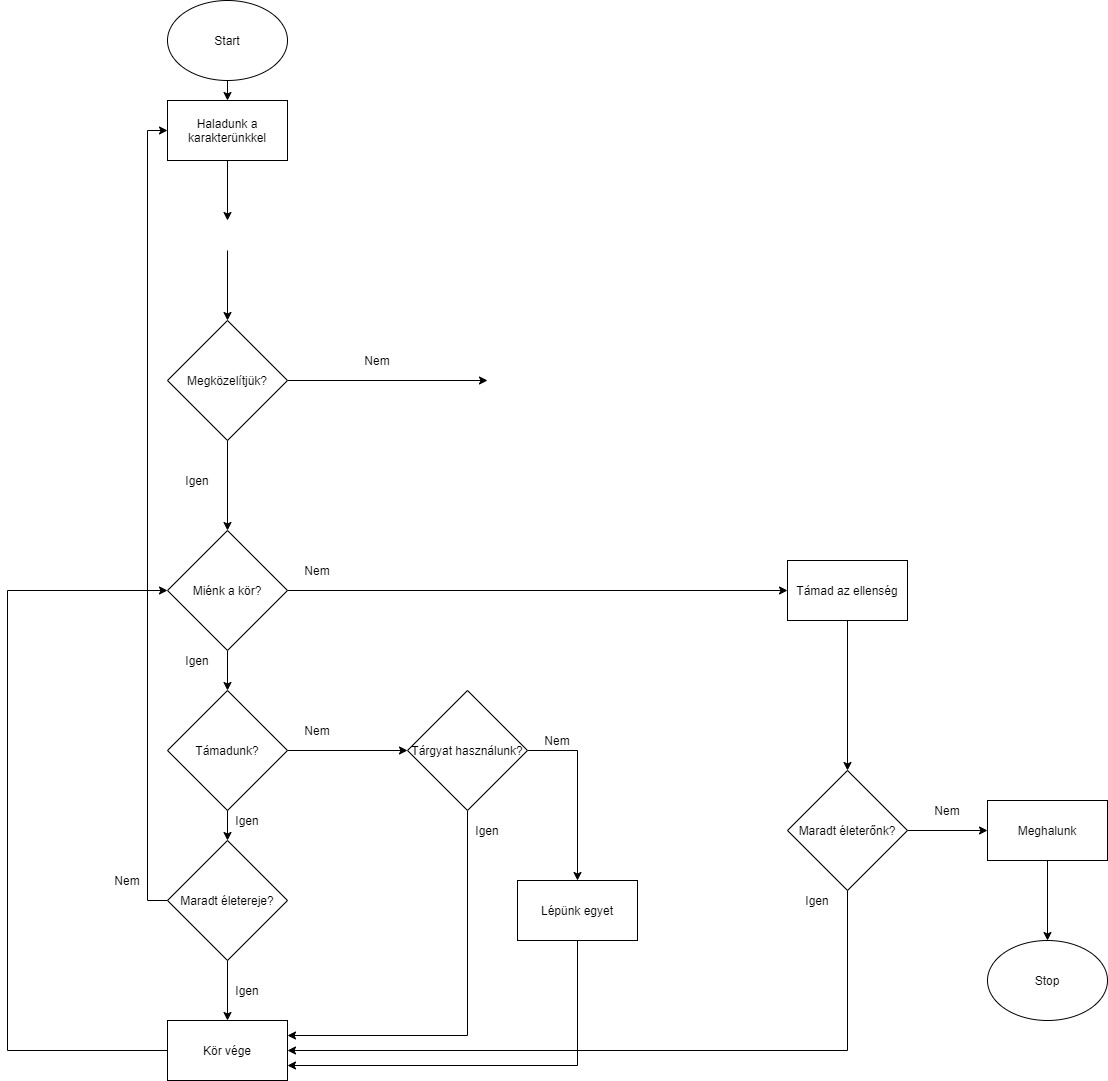
\includegraphics[width=\textwidth]{images/image5.png}
	\caption{Combat folyamatábra}
	\label{fig:combat2}
\end{figure}

\Section{Entity}

Egy blokk-on csak egy darab entity lehet, nem lehet rajtuk átmenni.
A játékon belül minden pozició intiger típussal van megadva.

% TODO: A platform itt most egy blokkot jelentene? -

% TODO: Az entity-k és a karakterek pozíciója milyen számtípussal van megadva?

\noindent No. 1. Entity:
\begin{itemize}
    \item Körönként 1 lépést tesz meg.
    \item Körönként 1 támadást hajt végre.
    \item Nagyobb kitérés.
    \item Ajtóban sebezhetőek az első támadásig.
    \item Halálukkor 5 tapasztalati pontot adnak.
\end{itemize}

\noindent No. 2. Entity:
\begin{itemize}
    \item Körönként 1 lépést tesz meg.
    \item Körönként 1 támadást hajt végre.
    \item Halálukkor 3 tapasztalati pontot adnak.
\end{itemize}

\noindent No. 3. Entity:
\begin{itemize}
    \item Körönként 3 lépést tesz meg.
    \item Körönként 3 támadást hajt végre.
    \item Halálukkor 4 tapasztalati pontot adnak.
\end{itemize}

\noindent No. 4. Entity:
\begin{itemize}
    \item Körönként 1 lépést tesz meg.
    \item Körönként 3 támadást hajt végre.
    \item Halálukkor 4 tapasztalati pontot adnak.
    \item Képes ranged attack-ok végrehajtására 3 blocknyi távolságból.
\end{itemize}

\noindent Egyéb:
\begin{itemize}
    \item Az Entytik elkerülik a rejtett csapdákat.
    \item Az Entytik 80\%-a alvó állapotba kerül be a szobák egyikébe és úgy is marad amíg meg nem közelíti a játékos az adott szobát.
    \item A többi nem alvó szabadon mozog, valahányszor mi is kört igénylő cselekvést hajtunk végbe.
\end{itemize}

\Section{Térbeli objektumok}

A térbeli objektumokra karakterünk nem képes rálépni, nem lát át rajtuk.
\begin{itemize}
\item
Ajtók: Karakterünk vagy egyéb entity-k az ajtó poziciójára lépnek akkor az ajtó kinyílik ha nem kulccsal zárt.
\item
Zárt ajtók: Rákattintunk és a karakterünk a közvetlen közelébe megy és van nálunk hozzá megfelelő kulcsunk akkor a karakterünk egy körért cserébe eltávolítja a zárt az ajtóról, ezek után sima ajtóként funkcionál.
\item
Kovácsműhely: Rákattintunk és a karakterünk a közvetlen közelébe megy, ha odaértünk akkor karakterünk interaktál vele és megnyílik egy felugró ablak. A felugró ablakon különböző akciókat hajhatunk végre. A szerzett alapanyagok segítségével tudjuk továbbfejleszteni a már meglévő felszereléseinket. Egy körbe kerül.

% TODO: A felugró ablakokról, és úgy általában a widget-ek kezeléséről érdemes részletesebben írni.

\item
Félkarú rabló: Rákattintunk és a karakterünk a közvetlen közelébe megy, ha odaértünk akkor karakterünk interaktál vele és megnyílik egy felugró ablak. Az általunk birtokolt aranyért cserébe esélyünk van játszani a félkarú rablón ami egy körbe kerül. A félkarú rabló nem mindig ad vissza tárgyat csak ha nyerünk vele. A nyeremény az az item amit 3-szor egymás után kipörget a játékos, egy játékon belül.

% TODO: Ennek megjelenítéséről érdemes lenne még írni, ábrát készíteni hozzá.

ábra{HAMAROSAN}

% TODO: A valószínűségeket konkretizálni kellene.

\item
Főzetfőző állomány: Rákattintunk és a karakterünk a közvetlen közelébe megy, ha odaértünk akkor karakterünk interaktál vele és megnyílik egy felugró ablak. Az általunk birtokolt növényi alapanyagok használatával fözetet készíthetünk, legalább 3 alapanyag szükséges hozzá. Az alapanyogtól függően van esély valamilyen típúsú főzet elkészítésére. Úgy működik, hogy: 3 alapanyagból, "a gép kihúz" egyet és amilyen az alapanyag, olyan lesz a főzet is. Lehet több ugyanolyan alapanyagot haszálni, ilyenkor nyílvánvalóan több esélyünk lesz az adott alapanyag "kihúzására". Hogyha 3 ugyanolyan alapanyagot használunk, akkor +40\%-kal hatékonyabb vagy hosszabb(főzettől függő).

% TODO: A véletlenszerű főzet itt bármi lehet, vagy függ egyéb tényezőtől is?

\item
Ércek: Rákattintunk és a karakterünk a közvetlen közelébe megy, ha odaértünk akkor karakterünk egy körért cserébe eltünteti a közvetlen közelünkben lévő ércet és kapunk egy alapanyagot.
\item
Láda: Rákattintunk és a karakterünk a közvetlen közelébe megy, ha odaértünk akkor karakterünk interaktál vele. A láda ezekután eltünik és egy tárgyat hagy hátra. Egy loot table-ben megadott tárgyak közül sorsolja ki, hogy milyen tárgyat hagy hátra. (később: táblázat)

% TODO: Az, hogy milyen tárgy, az mitől függ?

\item
Zárt láda: Rákattintunk és a karakterünk a közvetlen közelébe megy, ha odaértünk akkor karakterünk interaktál vele ha van hozzá megfelelő kulcs és a zárt láda átalakul sima ládává.
\item
Lépcsők: Rákattintunk és a karakterünk a közvetlen közelébe megy, ha odaértünk akkor karakterünk a következő szintre lép. Ilyenkor egy kisebb animáció történik, ahol a karakterünk lesétál a lépcsőn, és elsötétedik a kép.

% TODO: Ehhez tartozna majd valamilyen külön (modális) animáció is? -
\end{itemize}

\Section{Loot}

Az ellenfelek halál esetén \%-os eséllyel hagynak hátra maguk után valamilyen itemet.

A tárgyak amelyeket nem veszünk fel a játék végéig ott maradnak.

Minden entity más itemet hagyhat maga után.
Bizonyos térbeli elemek is adhatnak különböző itemeket.

Minden entitynek van egy loot táblája, amiben elő van írva, hogy milyen tárgyat hagyhat maga után milyen százalékos eséllyel.

% TODO: Az, hogy milyen tárgyakat hagynak hátra, az mitől függ? -

Bizonyos ládák illetve ajtók kulcsot, igényelhetnek.
Bármely entity dobhat aranyat, amelyet normális eloszlású RNG sorsol ki [20;70] intervallumon belül. Amit félkarú rablóknál is lehet elkölteni felszerelések fejlesztésére.

% TODO: A [20, 70] intervallumon belül hogy kerül meghatározásra az érték? -

Néhány alap szoba, folyosó blokkjainak felét fű borítja amelynek letaposásából \%-os eséllyel kaphatunk magvakat amiket el lehet ültetni ezzel csapdát állítva ellenfeleknek illetve szemgolyókat amik 1 életerőt gyógyítanak.

Alapfelszerelésen kívül minden felszerelés amit lootolunk számunkra ismeretlen felvételükkor 10 körig nem lehet levenni őket és a körök lejárta után pozitív vagy negatív effektet adnak.

Szemgolyókon kívül minden item amit lootolhatunk hatásuk számunkra ismeretlen első használatkor, a játék előrehaladtával ismerjük meg különböző tekercsek illetve főzetek effektjeit,a már egyszer használt itemek effektjeit karakterünk ismeri.

\Section{Itemek}

Az itemek a földről úgy vehetőek fel, hogy karakterünk arra a blokkra lép ahol az item található, ekkor megjelenik egy gomb amely rákattintásakor felveszi az itemet hogyha van hely az inventorynkban. Ha nincs hely, akkor mag a gomb szürkésebb. Ez a gomb a távolsági fegyver használati gombtól közvetlenül balra helykezedik el. Octagon alakú.

% TODO: Ezt a gombot is, mint widget-et részletezni kellene.

Az inventory mérete fix legyen 20 egység pl.: 4 egység széles 5 egység magas elosztásban.

Az inventoryból minden item egyetlen egy egységet igényel tárolásra.

Leltárban fix helye van az aranynak a jobb alsó sarokban.

Minden tárgyból bármekkora mennyiséget lehet tárolni.
Egyes objectek nem kerülnek az inventory-ba ennek oka hogy hatásukat kifejtik felvételükkör. (szemgolyók)

Entityk vagy térbeli elemek adják.
különböző felhasználási lehetőségekkel.
Fegyverek, Armorok.

Bizonyos stat növelők (Főzetek).
Minden tárgynak, amelyet Entitykből vagy térbeli objektumokból szerezhetőek meg, nem fix esélyű tárgyak.

\SubSection{Felszerelések}
%\label {subsec:Felszerelesek}

Felszerelésnek tekintjük az olyan állandó item-eket amelyeket fel lehet rakni karakterünkre.

Három altípusát különböztetjük meg a felszereléseknek:
\begin{itemize}
  \item Fegyverek
  \item Páncélok
  \item Ékszerek
\end{itemize}

Fegyverek feloszlanak 4 alkategóriára:
\begin{itemize}
  \item Kardok
  \item Íjak
  \item Varázsbotok
  \item Tőrök
\end{itemize}

Minden fegyver rendelkezik az alapvető támadó értéken kívül egy státusszal amely a ritkaságától függően eltérően ad %-osan támadóértéket.

Tehát karakterünk teljes támadóértékét a következőképpen tudjuk kiszámítani:

(BASE ATK+STRENGTH ATK+ITEM ATK)*WEAPON ATK percent=TOTAL ATK

A kapott érték alsó egészrészét vesszük minden alkalommal.

Ez a fajta számítás mind ékszereknél mind páncéloknál hasonlóan működik a különség csak  statisztákban van.

Fegyverek:
\begin{itemize}
  \item fegyver1
  \item fegyver2
  \item fegyver3
  \item fegyver4
  \item fegyver5
  \item fegyver6
  \item fegyver7
  \item fegyver8
  \item fegyver9
  \item fegyver10
  \item fegyver11
  \item fegyver12
\end{itemize}
\newpage
Ritkaság alapján:

\begin{table}[h]
\centering
\caption{Átlagos Fegyverek alapstatisztikái!}
\label{tab:minta}
\begin{tabular}{|l|c|c|c|c|}
\hline
 & fegyver1 & fegyver2 & fegyver3 & fegyver4 \\
\hline
Típus & Tőr & Kard & Varázsbot & Íj  \\
\hline
Alap támadóérték & 3 & 3 & 3 & 3 \\
\hline
Hatótáv & 1 & 1 & 3 & 3 \\
\hline
Támadás\% & 5 & 5 & 5 & 5 \\
\hline
\end{tabular}
\end{table}

\begin{table}[h]
\centering
\caption{Ritka Fegyverek alapstatisztikái!}
\label{tab:minta}
\begin{tabular}{|l|c|c|c|c|}
\hline
 & fegyver5 & fegyver6 & fegyver7 & fegyver8   \\
\hline
Típus & Tőr & Kard & Varázsbot & Íj  \\
\hline
Alap támadóérték & 5 & 5 & 5 & 5  \\
\hline
Hatótáv & 1 & 1 & 5 & 5 \\
\hline
Támadás\% & 10 & 10 & 10 & 10\\
\hline
\end{tabular}
\end{table}

\begin{table}[h]
\centering
\caption{Legendás Fegyverek alapstatisztikái!}
\label{tab:minta}
\begin{tabular}{|l|c|c|c|c|}
\hline
 & fegyver9 & fegyver10 & fegyver11 & fegyver12  \\
\hline
Típus & Tőr & Kard & Varázsbot & Íj\\
\hline
Alap támadóérték & 10 & 10 & 10 & 10 \\
\hline
Hatótáv & 1 & 1 & 8 & 8 \\
\hline
Támadás\% & 20 & 20 & 20 & 20 \\
\hline
\end{tabular}
\end{table}

\newpage

Péncélok alapstátusza:HP\% alapstatisztikája:védelem

Páncélok:

\begin{itemize}
  \item páncél1
  \item páncél2
  \item páncél3
  \item páncél4
  \item páncél5
  \item páncél6
  \item páncél7
  \item páncél8
  \item páncél9
  \item páncél10
  \item páncél11
  \item páncél12
\end{itemize}

\begin{table}[h]
\centering
\caption{Átlagos Páncélok alapstatisztikái!}
\label{tab:minta}
\begin{tabular}{|l|c|c|c|c|}
\hline
 & páncél1 & páncél2 & páncél3 & páncél4  \\
\hline
Típus & Acél & Bőr & Lánc & Szövet\\
\hline
Védelem & 10 & 10 & 10 & 10 \\
\hline
Életerő\% & 5 & 5 & 5 & 5 \\
\hline
\end{tabular}
\end{table}

\begin{table}[h]
\centering
\caption{Ritka Páncélok alapstatisztikái!}
\label{tab:minta}
\begin{tabular}{|l|c|c|c|c|}
\hline
 & páncél5 & páncél6 & páncél7 & páncél8  \\
\hline
Típus & Acél & Bőr & Lánc & Szövet\\
\hline
Védelem & 15 & 15 & 15 & 15 \\
\hline
Életerő\% & 10 & 10 & 10 & 10 \\
\hline
\end{tabular}
\end{table}

\begin{table}[h]
\centering
\caption{Legendás Páncélok alapstatisztikái!}
\label{tab:minta}
\begin{tabular}{|l|c|c|c|c|}
\hline
 & páncél1 & páncél2 & páncél3 & páncél4  \\
\hline
Típus & Acél & Bőr & Lánc & Szövet\\
\hline
Védelem & 25 & 25 & 25 & 25 \\
\hline
Életerő\% & 20 & 20 & 20 & 20 \\
\hline
\end{tabular}
\end{table}

\newpage
\noindent Ékszerekből maximum 2-őt tud hordani karakterünk.

4 fajtáját különböztetjük meg:

\begin{itemize}
  \item Gyűrűk
  \item Karkötők
  \item Nyakláncok
  \item Fülbevalók
\end{itemize}

\noindent Gyűrűk ATK\%-ot,Karkötők HP\%,Nyakláncok Crit rate\%,Fülbevalók Dodge\%-et adhatnak.

Ékszerek:

\begin{itemize}
 \item Gyűrű1
 \item Gyűrű2
 \item Gyűrű3
 \item Gyűrű4
 \item Karkötő1
 \item Karkötő2
 \item Karkötő3
 \item Karkötő4
 \item Nyaklánc1
 \item Nyaklánc2
 \item Nyaklánc3
 \item Nyaklánc4
 \item Fülbevaló1
 \item Fülbevaló2
 \item Fülbevaló3
 \item Fülbevaló4
\end{itemize}
\newpage
Típus alapján:

\begin{table}[h]
\centering
\caption{Gyűrűk alapstatisztikái!}
\label{tab:minta}
\begin{tabular}{|l|c|c|c|c|}
\hline
 & Gyűrű1 & Gyűrű2 & Gyűrű3 & Gyűrű4  \\
\hline
Ritkaság & Áltagos & Ritka & Epik & Legendás\\
\hline
Kritikus találat\% & 5 & 10 & 15 & 20 \\
\hline
\end{tabular}
\end{table}

\begin{table}[h]
\centering
\caption{Karkötők alapstatisztikái!}
\label{tab:minta}
\begin{tabular}{|l|c|c|c|c|}
\hline
 & Karkötő1 & Karkötő2 & Karkötő3 & Karkötő4  \\
\hline
Ritkaság & Áltagos & Ritka & Epikus & Legendás\\
\hline
Kitérés\% & 5 & 10 & 15 & 20 \\
\hline
\end{tabular}
\end{table}

\begin{table}[h]
\centering
\caption{Nyakláncok alapstatisztikái!}
\label{tab:minta}
\begin{tabular}{|l|c|c|c|c|}
\hline
 & Nyaklánc1 & Nyaklánc2 & Nyaklánc3 & Nyaklánc4  \\
\hline
Ritkaság & Áltagos & Ritka & Epikus & Legendás\\
\hline
Védelem\% & 5 & 10 & 15 & 20 \\
\hline
\end{tabular}
\end{table}

\begin{table}[h]
\centering
\caption{Fülbevalók alapstatisztikái!}
\label{tab:minta}
\begin{tabular}{|l|c|c|c|c|}
\hline
 & Fülbevaló1 & Fülbevaló2 & Fülbevaló3 & Fülbevaló4  \\
\hline
Ritkaság & Áltagos & Ritka & Epikus & Legendás\\
\hline
Életerő\% & 5 & 10 & 15 & 20 \\
\hline
\end{tabular}
\end{table}
\newpage

\SubSection{Kulcsok}

Minden mapon annyi kulcs spawnol, véletlenszerűen a szobák egyikébe amennyi kulcs\-csal zárt ajtó generálódott a mapra.
Kulcsok csak nyitott szobákba kerülnek generáláskor, így gátolva az esetleges 'lehetetlen' helyzeteket. Egy kizáró feltétel akadályozza meg.
% TODO: Itt hogyan garantálható, hogy egy szoba kulcsa ne abba a szobába kerüljön, amelyikkel be van zárva?

Láda Kulcsok:
Máshogy néznek ki grafikailag, mint a sima kulcs és külön vannak tárolva tőlük. Ezek a kulcsok a zárt ládák kinyitására használhatóak.
A Játékos felvételekor tisztában van azzal hogy az adott kulcsnak mi a szerepe, a nevéből és a leírásából kifolyólag.
% TODO: Érdemes lehet ezeket láda kulcsoknak hívni.

% TODO: A játékos tudja, hogy a felvett kulcs az ajtót vagy ládát nyit?

Ha a mapon van zárt láda, mindig 2 van vízszintesen és függőlegesen is legalább 1 blokknyi távolságra és maximum 2 blokknyi távolságra. És a mapra mindig csak 1 kulcs kerül hozzá.

% TODO: A közel itt mit jelent pontosan?

\SubSection{Alapanyagok}

Bizonyos felszerélesek fejlesztéséhez bizonyos alapanyagok szükségesek, ezeket megszerezhetjük ellenségektől vagy térbeli objektumokkal.
Ilyen térbeli objektum például egy érc, vagy egy növény.

A főzetek készítéséhez is szükségünk van alapanyagokra, ezeket szintén Entityk is dobhatják, de beszerezhetjük őket növényekből is.

\SubSection{Magvak}

Fűvel ellátott blokk letaposásából(az adott blokkra lépéssel) kaphatunk \%-os eséllyel.
Minden fű típusnak van egy loot táblája, ahol meg van adva melyik fű típus, milyen eséllyel, milyen itemet hagy hátra maga után.
% TODO: Az ilyen jellegű százalékokat hol és hogy kellene megadni?

Mindenfajta magvat el lehet dobni ilyenkor a magból kikelt növény hatása a helyétől körben 1 block távolságban fejti ki hatását 3 körig.

Magvak típusai:

\begin{itemize}
\item borotva: Eltiprásakor(rálépésekor) aktiválódik a hatása, ami az elültetés helyétől körben 1 blokknyi távolságra 3-at sebez az aktiválás utáni első körben.
\item gyógyító: Eltiprásakor(rálépésekor) aktiválódik a hatása, ami elültetés helyétől körben 1 blokknyi távolságra 3-at gyógyít az aktiválás utáni első körben.
\item mérgező: Eltiprásakor(rálépésekor) aktiválódik a hatása, ami elültetés helyétől körben 1 blokknyi távolságra méreg effektet rak az egységre amely 2 körön keresztül sebez 2-őt.
\end{itemize}

% TODO: A sebzés és gyógyítás kiértékelési sorrendjét érdemes vizsgálni!

\SubSection{Főzetek}

Játékban talált alapanyagokat összefőzhetjük egy adott főzőállomásnál, amely egy véletlenszerű hatású főzetet ad vissza nekünk.
Továbbá szimplán találhatunk szobákban ismeretlen főzeteket.
Minden főzetet el lehet dobni vagy meglehet inni, ilyenkor a becsapódás helyétől körben 1 block-nyira hat.

Főzetek típusai:
\begin{itemize}
\item Gyógyítás: A jelenlegi HP-nk 80\%-át visszatölti használatkor.
% TODO: A számításokkal kapcsolatban érdemes részletezni a kerekítési szabályokat is.
\item Mérgezés: Megmérgez minket, amely körönként 3 sebzést okoz, 3körig. Ellenségre is lehet dobni.
\item Altató: Elaltat minket 3körig, ellenségre is alkalmazható.
\item Azonnali sebzés: Használatkor azonnal sebez 30\%-ot a maximum HP-ból. Ellenségre is alkalmazható.
\item Teleport: Használatkor elteleportálja a karakterünket véletlenszerű helyre a mapon belül, eldobáskor maximum 3 entityt, saját magunkat beleszámolva telepíthet el, több különböző helyre.
\item Felderítő: Minden szobát úgy látunk, mintha már lettünk volna ott előzőleg. Véglegesen.
\item Lebegés: Csapdákat, vizes területeket, kerülhetünk el használatkor. 10 körig tart a hatása.
\end{itemize}

\Section{Idő}

A szobán belülre kattintva odamegy a karakter ahova kattintunk, ha nem fedezz fel új ellenséget, ha mégis akkor megáll.

Az ellenfeleknek annyi akciója van amennyi akciót elvégeztünk a karaktereinkkel és velünk párhuzamosan cselekednek.

Az idő csak akkor telik amikor karakterünk végrehajt valamilyen akciót.Akciónak számít a mozgás, keresés, támadás, védekezés, tárgy használata.

\Section{Kamera}

Legyen a fény forrása a karakter, az adott szobában, nagyságától függetlenül minden ki van világítva, hogyha nem akadályozza semmi a fény útját.
A szobákat mindig felülnézetben láthatjuk, ahol a kamera leköveti a karakter mozgását, úgy hogy mindig középen legyen az.
A bal egérgomb letartásával és egér mozgatásával tudjuk mozgatni a kamerát.

\begin{figure}[h!]
	\centering
	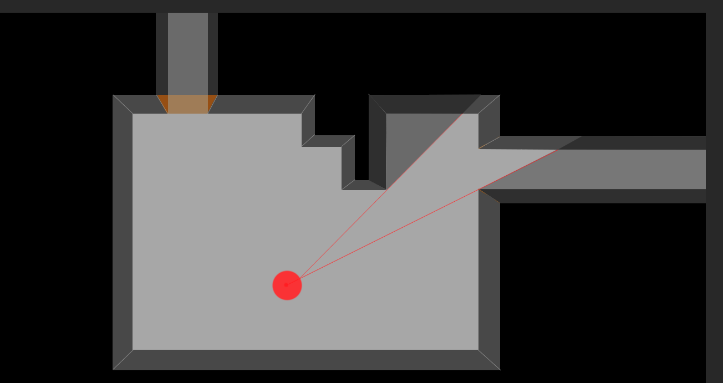
\includegraphics[scale=1]{images/image6.png}
	\caption{Kamera 1}
	\label{fig:camera1}
\end{figure}

\begin{figure}[h!]
	\centering
	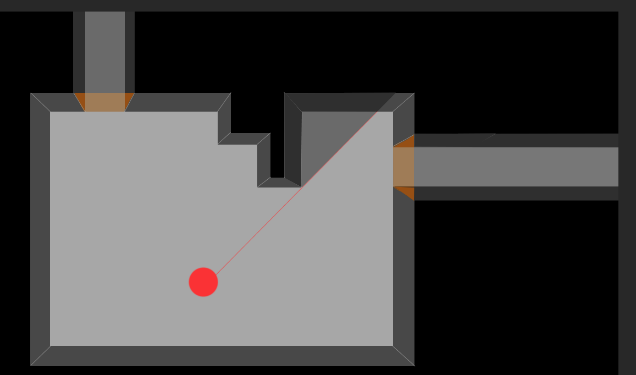
\includegraphics[scale=1]{images/image7.png}
	\caption{Kamera 2}
	\label{fig:camera2}
\end{figure}

\Aref{fig:camera1}. és \aref{fig:camera2}. ábrákon láthatunk egy szobát amelyben a karakterünk van (piros gömb), a fény arra terjed amerre a karakterünk forogna,ellátna.
Az ajtók ha nyitva vannak a fény továbbterjed a folyosóra.

A már előzőlegesen látott területek, látszódnak akkor is ha a karakterünk nem lát rá, annyi különbséggel, hogy az adott területen lévő változók nem változnak számunkra (pl: az adott területen van egy fű típus egy blokkon, amit egy entity letapos, ha a ezt a fű típust akkor láttuk amikor még nem volt eltaposva, akkor úgy is fogjuk látni, amíg nem látunk újra rá), illetve az adott területen áthaladó ellenfeleket se látjuk.
Az előzőlegesen nem látott területeket, sehogy se látjuk, kivétel ha valamilyen tárggyal felderítjük azt (pl: főzet).

% TODO: Az árnyékos részen hogyan látszódnak az ellenfelek és a felvehető tárgyak? -

% TODO: A bejárt és a még be nem járt területek között van különbség láthatóság szempontjából? -

\Section{Irányítás}

A kurzor használatával az adott területre kattintva halad oda a karakter.
Bizonyos helyezetekben megjelenő gombokra kattintva bizonyos tevékenységek lebonyolítása.
Egyéb menü/inventory megjelenítés bizonyos gombok segítségével(Esc,I, stb…)
A már általunk felfedezett területre kattintva karakterünk a lehető leggyorsabb útvonalat választja.
A mozgás a felengedésre aktiválódik.
A művelet végrehajtása közben, ha egy új műveletet kezdeményezünk akkor az előzőleges esemény félbeszakad abban a pillanatban, amikor felengedjük a gombot.

% TODO: Az esemény a lenyomásra vagy a felengedésre aktiválódik? -

% TODO: Egy műveletet vissza lehet vonni annak végrehajtása közben? -

\Section{Az interface-n megjelenő gombok}

\SubSection{Tárgyfelvételi gomb}

\begin{itemize}
    \item prekondíció:A karakterünk egy tárgy helyén áll.
    általános müködés: Az egeret rávisszük a tárgyfelvételnek szánt gombra, és bal egérgombbal rákattintunk.
    \item alternatív esetek: Több item van egyhelyen, egyszerre csak egy itemet veszünk fel.
    \item postkondíció: Az item bekerült az inventorynkba.
    kivételes esetek: Nincs hely az inventoryban új tárgy felvételéhez.
\end{itemize}

\SubSection{Menü}

\begin{itemize}
    \item prekondíció: Játékmenetben vagyunk.
    általános működés: Az egeret rávisszük a menünek szánt gombra, és bal egérgombbal rákattintunk.
    \item alternatív esetek: Rossz ablak nyílik meg, nem pedig a menü, például az inventory.
    \item Postkondíció: Megnyílt a menü, válaszhatunk, hogy mit szeretnénk továbbá megnyitni. Az ablak jobb felső sarkában lévő X gombra kattintva visszatérünk a játékba.
    \item kivételes esetek: Nem nyílt meg a menü, bal egérgomb kattintásával.
\end{itemize}

\SubSection{Inventory}

\begin{itemize}
    \item prekondíció: Játékmenetben vagyunk.
    \item általános működés: : Az egeret rávisszük az inventorynak szánt gombra, és bal egérgombbal rákattintunk.
    \item Postkondíció: Megnyílt az inventory, válaszhatunk, hogy az inventoryban tárolt tárgyak közül melyikkel lépünk kapcsolatba. Az ablak jobb felső sarkában lévő X gombra kattintva visszatérünk a játékba.
    alternatív esetek: Rossz ablak nyílik meg, nem pedig az inventory, például a karakter.
    \item kivételes esetek: Nem nyílt meg az inventory, bal egérgomb kattintásával.
\end{itemize}

\SubSection{Íj}

\begin{itemize}
    \item prekondíció: Játékmenetben vagyunk.
    általános működés: : Az egeret rávisszük az íjnak szánt gombra, és bal egérgombbal rákattintunk.
    \item Postkondíció: Ha van ellenség adott távolságon belül, akkor megjelenik a legközelebbi ellenfelen egy célkereszt, amely után, ha rákattintunk, végbe megy a támadás. Ha nincs ellenség, nincs célkereszt.
    Lőttünk vagy abbahagytuk az adott cselekvést, a kurzor visszaalakul.
    \item alternatív esetek: Nincs nyíl a karakternél, nem megy végbe a támadás.
    \item kivételes esetek: Nem vált át íjra a karakter. Hiába kattintunk a gombra.
\end{itemize}

\SubSection{Súgó}

\begin{itemize}
    \item prekondíció: Játékmenetben vagyunk.
    általános működés: Az egeret rávisszük a súgónak szánt gombra, és bal egérgombbal rákattintunk.
    \item Postkondíció: : Ha a játékon belüli objectre kattintunk, akkor megjelenik egy felugró ablakban az adott object rövid leírása. Az ablak jobb felső sarkában lévő X gombra kattintva visszatérünk a játékba.
    \item alternatív esetek: Nem annak az objectnek jelenik meg a leírása, mint amire rákattintottunk.
    \item kivételes esetek: Nincsen elérhető információ az adott objectről.
\end{itemize}

\SubSection{keresés}

\begin{itemize}
    \item prekondíció: Játékmenetben vagyunk.
    általános működés: : Az egeret rávisszük a keresésnek szánt gombra, és bal egérgombbal rákattintunk.
    \item Postkondíció: Megjelennek a karakterünk közvetlen közelében lévő rejtett objectek. Például rejtett ajtó/csapda. Az ablak jobb felső sarkában lévő X gombra kattintva visszatérünk a játékba.
    \item alternatív esetek: Nem az a funkció megy végbe, amelyet szerettünk volna.
    \item kivételes esetek: Nem jelenik meg, hiába kéne megjelennie keresés után az adott objectnek.
\end{itemize}

\SubSection{Karakter}

\begin{itemize}
    \item prekondíció: Játékmenetben vagyunk.
    általános működés: Az egeret rávisszük a karakternek szánt gombra, és bal egérgombbal rákattintunk.
    \item Postkondíció: Megjelenik 4 különböző lehetőség, hogy mit fejlesszünk a karakterünkön amelyek akkor mennek végbe ha van hozzá elegendő pontunk. Az ablak jobb felső sarkában lévő X gombra kattintva visszatérünk a játékba.
    \item alternatív esetek:Nem a mi karakterünk jelennek meg az információk.
    \item kivételes eset:Nem jön elő a felugró ablak.
\end{itemize}
